\chapter{Extras}
\label{Extras}
Unter bem Men�punkt \textit{Extras} werden verschiedenen Verwaltungstools zusammengefasst.
\section{Reihungstestverwaltung}
\begin{figure}
	\centering
	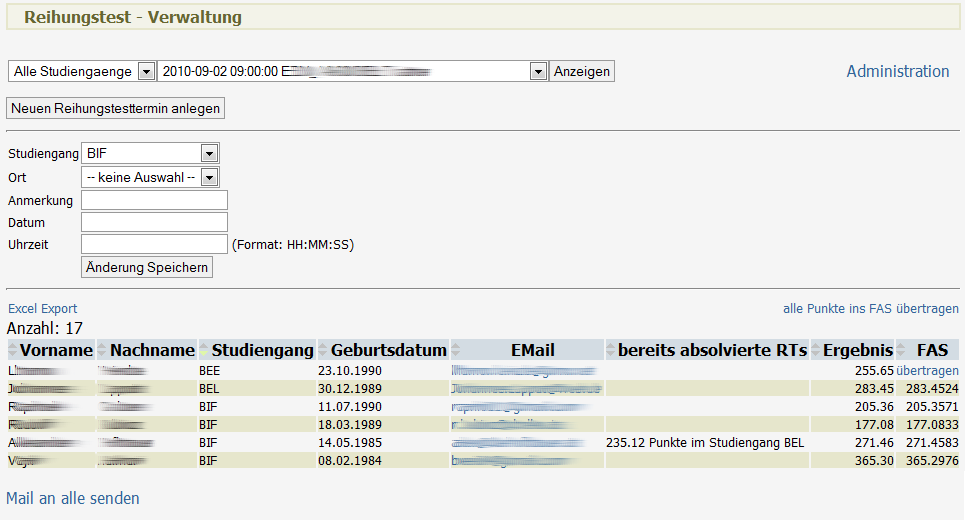
\includegraphics[width=0.75\textwidth]{FAS_Reihungstest1.png}
	\caption{Reihungstestverwaltung}
	\label{Reihungstest1}
\end{figure}
Mit dem Men�punkt \textit{Reihungstestverwaltung} wird das in Abbildung \ref{Reihungstest1} gezeigte Eingabeformular aufgerufen, mit dem neue Reihungstests angelegt und bestehende ver�ndert werden k�nnen.\\
Aufbau des Formulars:
\begin{itemize}
	\item Bereich 1: 	
	\begin{itemize}
		\item Auswahl Studiengang
		\item Auswahl Reihungstest: Das Angebot wird durch die Auswahl eines Studiengangs bestimmt.
		\item Button \textit{Anzeigen}: Anzeige der getroffenen Auswahl im Bereich 3.
		\item Button \textit{Neuen Reihungstesttermin anlegen}: Beginn der Eingabe eines neuen Reihungstests.
	\end{itemize}
	\item Bereich 2: 
	Die hier gruppierten Eingabefenster dienen zur Eingabe (Button \textit{Neuen Reihungstermin anlegen} wurde zuvor angeklickt) oder �nderung (Reihungstest wurde im Bereich 1 ausgew�hlt) von Reihungstestdaten:
	\begin{itemize}
		\item Studiengang
		\item Ort 
		\item Anmerkung
		\item Datum
		\item Uhrzeit
	\end{itemize}
	\item Bereich 3: 
	Das ist der Anzeigebereich der Teilnehmer am ausgew�hlten Reihungstest. Es besteht die M�glichkeit die Liste im Excel-Format anzuzeigen und zu speichern und ein E-Mail an alle Teilnehmer zu schicken. Weiters k�nnen hier die Reihungstestpunkte von allen bzw einzelnen Personen ins FAS �bertragen werden. 
\end{itemize}
\section{Firmenverwaltung}
siehe Kapitel \ref{Firmenverwaltung}
\section{Lehrveranstaltungverwaltung}
siehe Kapitel \ref{lehrveranstaltung}
\section{Projektarbeitsbenotung}
\begin{figure}
	\centering
	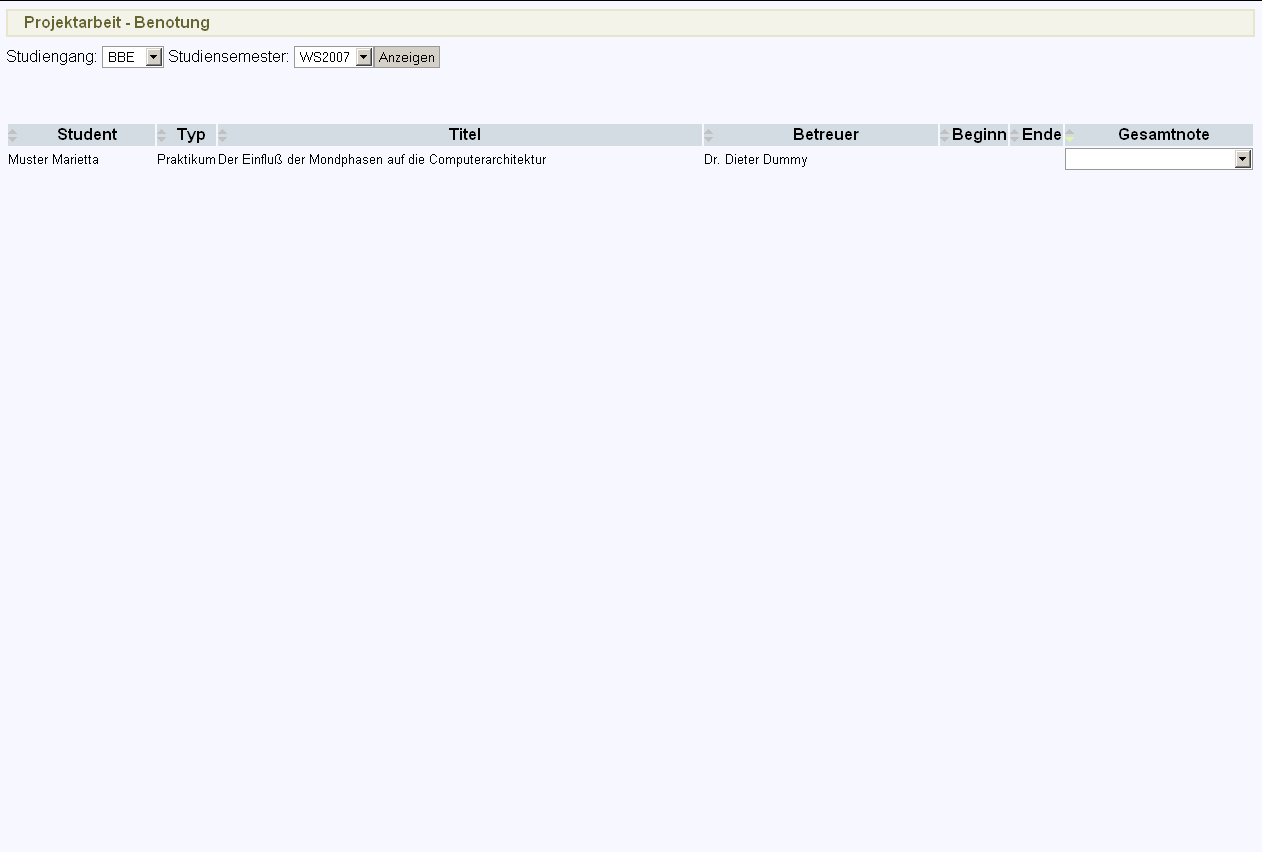
\includegraphics[width=0.75\textwidth]{FAS_Projektarbeitbenotung1.png}
	\caption{Projektarbeitbenotung}
	\label{Projektarbeitbenotung1}
\end{figure}
Hier wird das unter Abbildung \ref{Projektarbeitbenotung1} gezeigte Formular aufgerufen. Nach Auswahl von Studiengang und Studiensemester werden durch Klicken des Button \textit{Anzeigen} die betreffenden Projektarbeiten aufgelistet. Nun k�nnen die Noten der Projektarbeiten ausgew�hlt werden.
\section{Gruppenverwaltung}
Mit diesem Tool ist es m�glich \underline{bestehende} Gruppen zu aktivieren oder zu deaktivieren und die Bezeichnungen zu ver�ndern. \\
\underline{Beispiel}:
Zu Semesterbeginn soll ein neuer Incoming XY angelegt werden. Zuerst wird der Incoming, wie in Kapitel \ref{Incoming} Incoming beschrieben, angelegt. Der neue Incoming wird dem Lehrverband 0I zugeteilt. Da aber Incoming selten die gleichen Lehrveranstaltungen besuchen, k�nnen sie durch Gruppen getrennt werden. Deshalb wird im Karteireiter \textit{Details} des Incoming XY die Gruppe eingetragen, in 